\documentclass{article}
\usepackage{graphicx} % Required for inserting images
\usepackage{amsmath}
\usepackage{pgfplots}
\usepackage{tikz}
\usetikzlibrary{angles,quotes}

\title{Frames and Transformations}
\author{Intro to Robotics}
\date{}
\begin{document}

\maketitle

\section{Frames}
\textbf{Notation: } Let frame \{A\} be the universal coordinate system, and frame \{B\} = \{ ${}^{A}_{B}R_\theta$, ${}^{A}P_{Borg}$ \}\\
Where ${}^{A}P_{Borg}$ is the origin of frame \{B\} relative to frame \{A\}, and ${}^{A}_{B}R_\theta$ is the orientation of frame \{B\} relative to frame \{A\}.  \\\\
Below let A be the universal frame, and\\ 
frame \{B\} = \{ ${}^{A}_{B}R_{45^\circ}=$$\begin{bmatrix}
.707 & -.707 \\
.707 & .707
\end{bmatrix}$, 
${}^{A}P_{Borg}=$$\begin{bmatrix}
1 \\
2
\end{bmatrix}$ \}

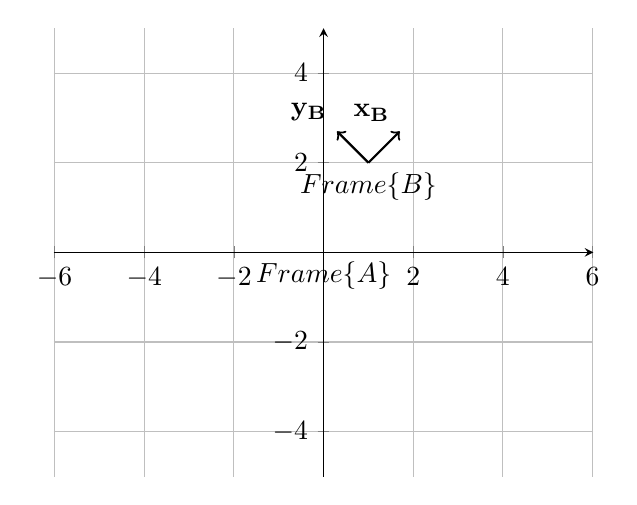
\begin{tikzpicture}
\begin{axis}[axis lines=middle, xmin=-5, xmax=5, ymin=-5,ymax=5,axis equal,grid=both]
\addplot [->, thick,  black] coordinates { (1,2) (1.7,2.7)}node[above left]{$\mathbf{x_B}$};
\addplot [->, thick,  black] coordinates { (1,2) (.3,2.7)}node[above left]{$\mathbf{y_B}$};
\addplot [black] coordinates { (1,2) (1,2)}node[below]{$Frame \{B\}$};
\addplot [black] coordinates { (0,0) (0,0)}node[below]{$Frame \{A\}$};
\end{axis}
\end{tikzpicture}\\

\subsection{2D rotation matrix}
\textbf{Note in this class we will always use degrees unless stated otherwise.}\\
In order to rotate frames and vectors we must introduce the 2D rotation matrix. The 2D rotation matrix allows us to easily rotate vectors and frames by simple matrix multiplication. The formula for the 2D rotation matrix is:\\
$R=\begin{bmatrix}
cos(\theta) & -sin(\theta) \\
sin(\theta) & cos(\theta)
\end{bmatrix}$ \\\\
\textbf{Example of rotating a vector:(make sure to use calculator in degree mode)}\\
Given vector $v_1 = \begin{bmatrix}
2 \\
2
\end{bmatrix}$ rotate it by $60^\circ$.\\\\
$Rv_1=\begin{bmatrix}
cos(60^\circ) & -sin(60^\circ) \\
sin(60^\circ) & cos(60^\circ)
\end{bmatrix}
\begin{bmatrix}
2 \\
2
\end{bmatrix}=
\begin{bmatrix}
.5 & -.87 \\
.87 & .5
\end{bmatrix}
\begin{bmatrix}
2 \\
2
\end{bmatrix}=
\begin{bmatrix}
-.74 \\
2.74
\end{bmatrix}=v_{1r}$\\\\

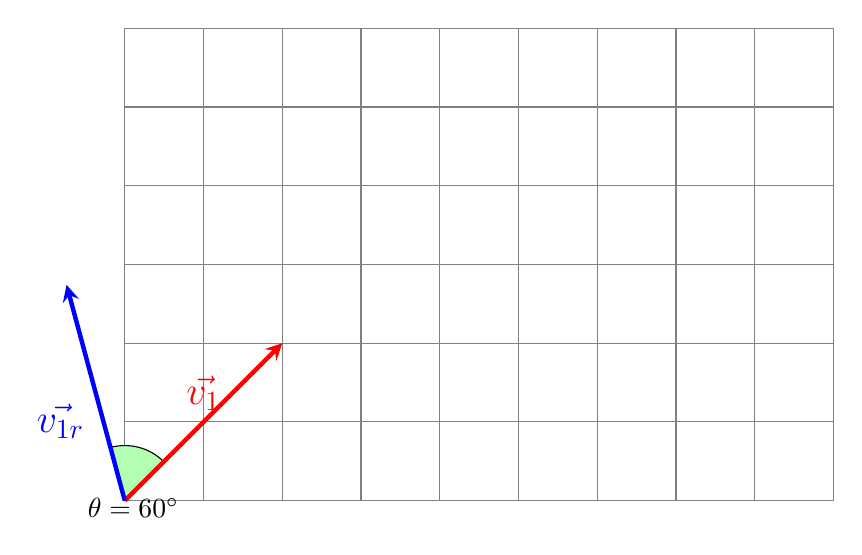
\begin{tikzpicture}[> = stealth]
\coordinate (a) at (0,0);
\coordinate (b) at (2,2);
\coordinate (c) at (-.74,2.74);

\draw[gray,step=1cm] (0,0) grid +(9cm,6cm);
%\draw pic[draw,fill=green!30,angle radius=1cm,"$\alpha$" shift={(6mm,1mm)}] {angle=c--a--b};
\draw pic[draw,fill=green!30,angle radius=0.7cm,"$\theta=60^\circ$" shift={(0mm,-5mm)}] {angle=b--a--c};

\draw[ultra thick,red, ->]  (a) -- node[above] {\Large $\vec{v_1}$} (b);
\draw[ultra thick,blue,->]  (a) -- node[below left] {\Large $\vec{v_{1r}}$} (c);
\end{tikzpicture}\\\\
\textbf{Note: A positive angle is a counterclockwise rotation, and a negative angle is clockwise rotation.}\\\\
\textbf{Notation: } ${}^A_BR$: Is the rotation from frame \{A\} to frame \{B\}(frame \{B\} relative to frame \{A\}).\\\\
Rotation matrices have special properties that apply to both 2D and 3D space.\\
\textbf{1.} Rotation matrices are orthonormal, which means the column vectors are all orthogonal, and have magnitude equal to 1.\\
\textbf{2.} Given $R_{\theta}$, then $R_{-\theta}=R_{\theta}^T=R_{\theta}^{-1}$, in other words, the transpose of a matrix is equal to its inverse. Which means if you rotate a vector by $\theta$ you can undo the rotation by multiplying by the transpose matrix.\\
\textbf{3.} The determinant of $R$ is always equal to 1 or -1.
\newpage
\section{Homogeneous Coordinates}
Using homogeneous coordinates we can represent the transformation of one frame into another.\\
\textbf{Notation: } ${}^A_BT$: Is the matrix that represents the transformation of frame \{A\} to frame \{B\}(frame \{B\} relative to frame \{A\}). This transformation applies a rotation followed by a translation. \\\\
The formula for generating matrix ${}^A_BT=\begin{bmatrix}
{}^A_B R & {}^A P_{Borg}\\
0 & 0 & 1
\end{bmatrix}$\\\\
\textbf{Example: }\\
Below let A be the universal frame, and\\ 
frame \{B\} = \{ ${}^{A}_{B}R_{60^\circ}=\begin{bmatrix}
cos(60^\circ) & -sin(60^\circ) \\
sin(60^\circ) & cos(60^\circ)
\end{bmatrix}=\begin{bmatrix}
.5 & -.867 \\
.867 & .5
\end{bmatrix}, 
{}^{A}P_{Borg}=\begin{bmatrix}
-3 \\
2
\end{bmatrix}$ \}\\\\
Then the homogeneous transformation matrix is ${}^A_B T = \begin{bmatrix}
{}^A_B R & {}^A P_{Borg}\\
0 & 0 & 1
\end{bmatrix}=\begin{bmatrix}
.5 & -.867 & -3 \\
.867 & .5 & 2 \\
0 & 0 & 1
\end{bmatrix}$

\subsection{Inverse of T}
The inverse of ${}^A_B T$ must satisfy the equation: ${}^A_B T {}^A_B T^{-1} = I$ where $I$ is the identity matrix. We know that ${}^A_B T$ is the transformation from frame \{A\} to frame \{B\}. So it follows that the inverse of ${}^A_B T$ "undoes" this transformation. In other words, ${}^A_B T^{-1}$ is the transformation from frame \{B\} to frame \{A\} and can be denoted as: \\\\${}^B_A T={}^A_B T^{-1}$. 
\newpage

To compute the inverse we use: \\\\
${}^A_B T^{-1}={}^B_A T=\begin{bmatrix}
{}^A_B R^T & -({}^A_B R^T {}^A P_{Borg}) \\
0 & 0 & 1
\end{bmatrix}$\\
We can derive this formula by applying RREF to the general case of ${}^A_B R^T$. \\\\
\textbf{Example: }\\
consider ${}^A_B T = \begin{bmatrix}
{}^A_B R & {}^A P_{Borg}\\
0 & 0 & 1
\end{bmatrix}=\begin{bmatrix}
.5 & -.867 & -3 \\
.867 & .5 & 2 \\
0 & 0 & 1
\end{bmatrix}$ \\\\
then its inverse matrix must be equal to:\\
${}^A_B T^{-1}={}^B_A T=\begin{bmatrix}
{}^A_B R^T & -({}^A_B R^T {}^A P_{Borg}) \\
0 & 0 & 1
\end{bmatrix}=\begin{bmatrix}
.5 &.867 & -(.5*-3 +.867*2 )\\
-.867 & .5 & -(-.867*-3 + .5*2) \\
0 & 0 & 1
\end{bmatrix}=\begin{bmatrix}
.5 &.867 & -.234 \\
-.867 & .5 & -3.601\\
0 & 0 & 1
\end{bmatrix}$\\\\
Now we can verify that ${}^A_B T {}^B_A T = I$ \\
$\begin{bmatrix}
.5 & -.867 & -3 \\
.867 & .5 & 2 \\
0 & 0 & 1
\end{bmatrix}
\begin{bmatrix}
.5 &.867 & -.234 \\
-.867 & .5 & -3.601\\
0 & 0 & 1
\end{bmatrix}=\begin{bmatrix}
1 & 0 & 0 \\
0 & 1 & 0 \\
0 & 0 & 1
\end{bmatrix}$

\section{Homogeneous transformations to rotate and translate vectors}
There are two ways to use transformations, the first way is to construct transformations to rotate and translate a vector. Let us demonstrate via example: \\
\textbf{Example: }\\
Given vector $P_1=\begin{bmatrix}
2\\
-4
\end{bmatrix}$ rotate it by $30^\circ$ and translate it by $t=\begin{bmatrix}
5 \\
-5
\end{bmatrix}$.
We can use homogeneous transformations to rotate then translate vectors(order matters we rotate then translate). We accomplish this by using: \\
$T P_i = \begin{bmatrix}
R_\theta & t\\
0 & 0 & 1
\end{bmatrix}\begin{bmatrix}
P_{i1}\\
P_{i2}\\
P_{i3}
\end{bmatrix}= P'_{i}$ where $P'_{i}$ is $P_i$ after rotation then translation.\\ so we get: $\begin{bmatrix}
cos(30^\circ) & -sin(30^\circ) & 5\\
sin(30^\circ) & cos(30^\circ) & -5\\
0 & 0 & 1
\end{bmatrix}\begin{bmatrix}
2\\
-4\\
1
\end{bmatrix}=\begin{bmatrix}
8.74\\
-7.48\\
1
\end{bmatrix}=P'_{i}$\\
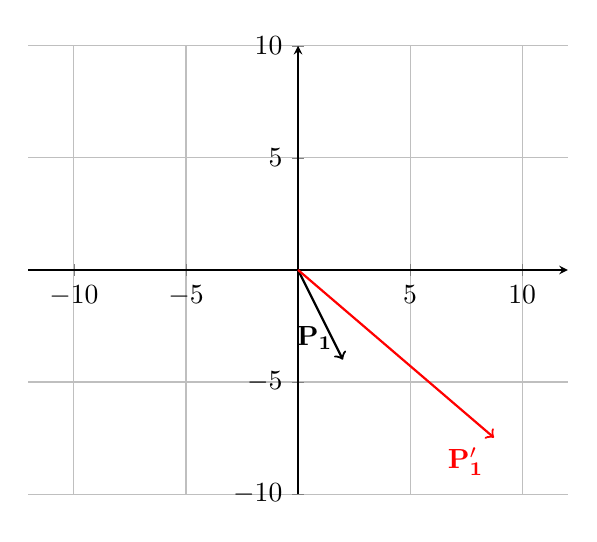
\begin{tikzpicture}
\begin{axis}[axis lines=middle, xmin=-10, xmax=10, ymin=-10,ymax=10,axis equal,grid=both]
\addplot [->, thick,  black] coordinates { (0,0) (2,-4)}node[above left]{$\mathbf{P_1}$};
\addplot [->, thick,  red] coordinates { (0,0) (8.74,-7.48)}node[below left]{$\mathbf{P'_1}$};
\end{axis}
\end{tikzpicture}

\newpage
\section{Using homogeneous transformations to communicate points across frames}
\textbf{Notation:}\\
\begin{figure}[htp]
    \centering
    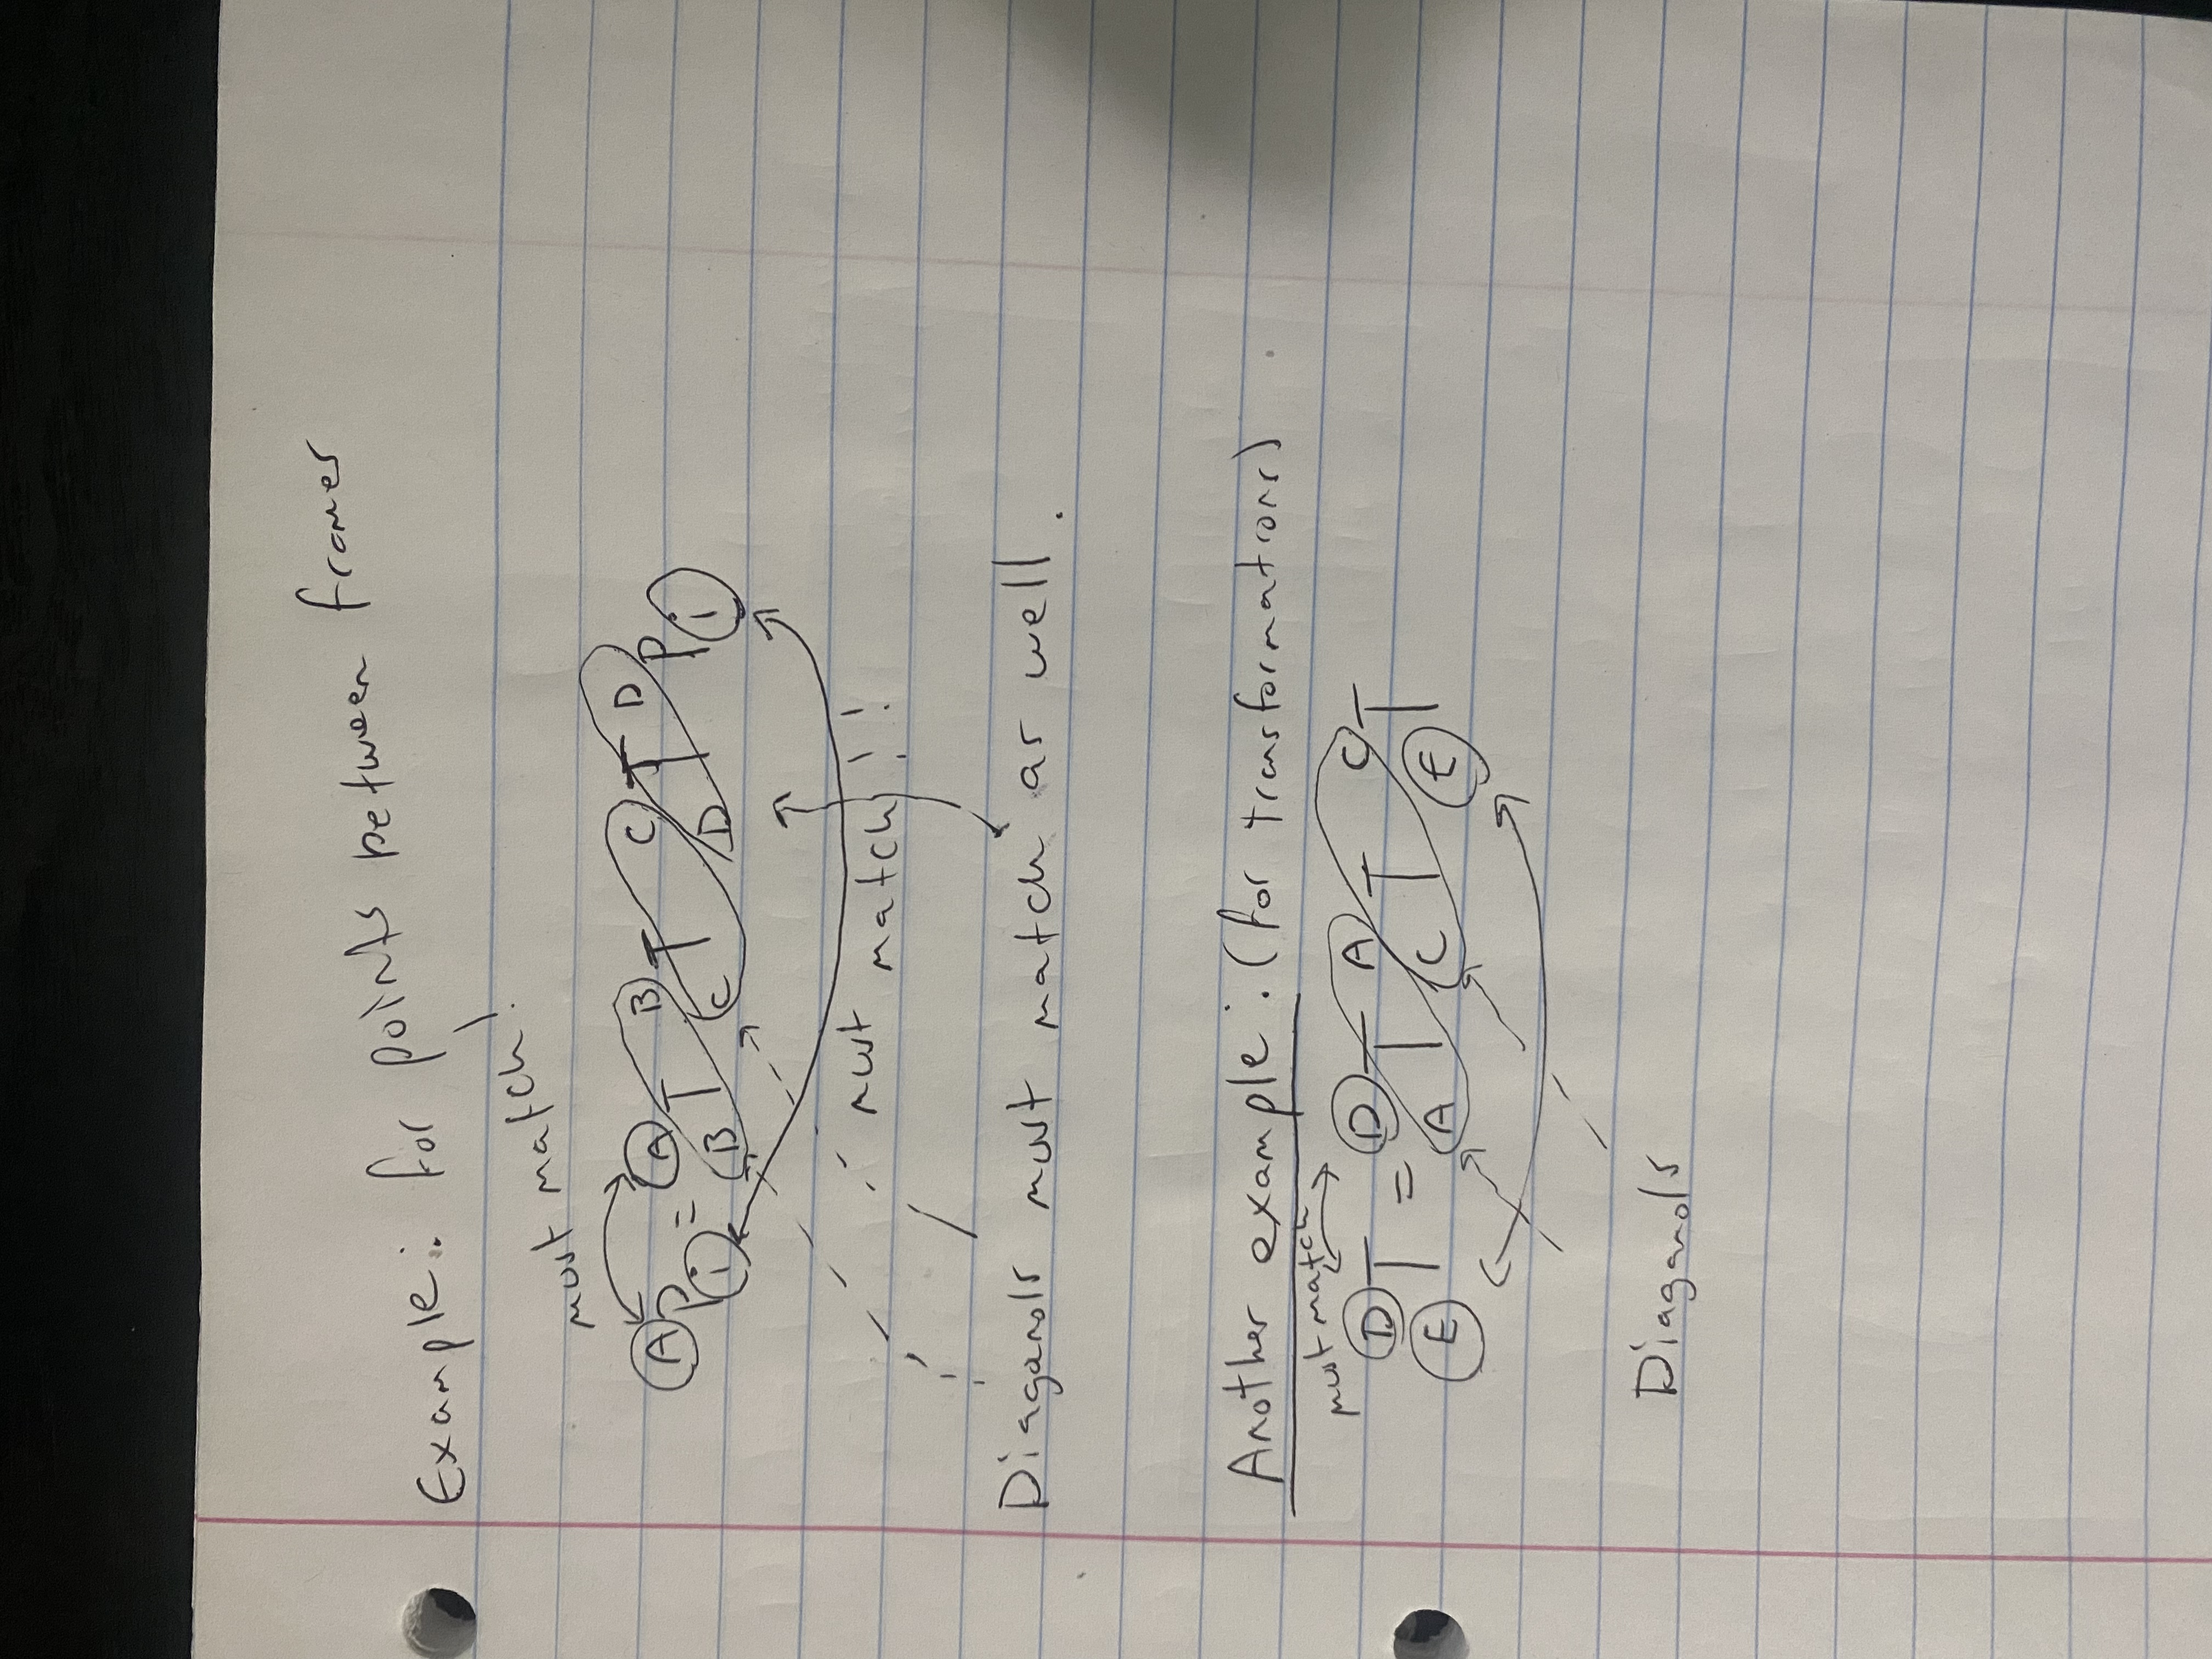
\includegraphics[width=12cm, angle =270 ]{notation.jpeg}
    \caption{}
    \label{fig:pubsub}
\end{figure}\\\\
\newpage
\textbf{Big Example: }\\    
Given frames: Frame \{A\} = universe,\\ 
Frame \{B\} = \{${}^{A}_{B}R_{70^\circ} ,{}^{A}P_{Borg}=\begin{bmatrix}
2 \\
1 
\end{bmatrix} $\},\\
Frame \{C\} = \{${}^{A}_{C}R_{100^\circ} ,{}^{A}P_{Corg}=\begin{bmatrix}
-3  \\
2 
\end{bmatrix} $\},\\
Frame \{D\} = \{${}^{C}_{D}R_{35^\circ} ,{}^{C}P_{Dorg}=\begin{bmatrix}
-1  \\
-1 
\end{bmatrix} $\}\\\\
Given points: ${}^{A}P_{1}=\begin{bmatrix}
4  \\
-3 
\end{bmatrix}$, ${}^{B}P_{2}=\begin{bmatrix}
2  \\
5 
\end{bmatrix}$, ${}^{C}P_{3}=\begin{bmatrix}
1  \\
6 
\end{bmatrix}$, ${}^{D}P_{4}=\begin{bmatrix}
1  \\
-1
\end{bmatrix}$\\
\textbf{The left superscript of the vector is the frame it is in, which means that the starting point of the vector is the origin of the frame it is in. }
\newpage
\textbf{0. Draw frames and vectors}\\
\begin{tikzpicture}[scale=2]
\begin{axis}[axis lines=middle, xmin=-10, xmax=10, ymin=-10,ymax=10,axis equal,grid=both]
\addplot [black] coordinates { (0,0) (0,0)}node[below]{$\{A\}$};
\addplot [->, thick,  red] coordinates { (0,0) (4,-3)}node[below]{$\mathbf{^A P_1}$};

\addplot [->, thick,  black] coordinates { (2,1) (2.34,1.94)}node[above left];
\addplot [->, thick,  black] coordinates { (2,1) (1.06,1.34)}node[above left];
\addplot [black] coordinates { (2,1) (2,1)}node[below]{$\{B\}$};
\addplot [->, thick,  red] coordinates { (2,1) (-2.02,4.58)}node[above left]{$\mathbf{^B P_2}$};

\addplot [->, thick,  black] coordinates { (-3,2) (-3.17,2.98)}node[above left];
\addplot [->, thick,  black] coordinates { (-3,2) (-3.98,1.83)}node[above left];
\addplot [black] coordinates { (-3,2) (-3,2)}node[below]{$\{C\}$};
\addplot [->, thick,  red] coordinates { (-3,2) (-9.05,1.96)}node[above left]{$\mathbf{^C P_3}$};

\addplot [->, thick,  black] coordinates { (-1.85,1.19) (-2.56,1.9)}node[above left];
\addplot [->, thick,  black] coordinates { (-1.85,1.19) (-2.56,.48)}node[above left];
\addplot [black] coordinates { (-1.85,1.19) (-1.85,1.19)}node[below]{$\{D\}$};
\addplot [->, thick,  red] coordinates { (-1.85,1.19) (-1.85,2.59)}node[above]{$\mathbf{^D P_4}$};
\end{axis}
\end{tikzpicture}\\

\textbf{1. Find} $\mathbf{{}^A_D T}$.\\\\
You must solve for $^A_DT$ by constructing a chain of transformations that gives $^A_DT$ according to the notation rules.\\
${}^A_D T=^A_C T {}^C_D T=^A_C T {}^C_D T=\begin{bmatrix}
c100 & -s100 & -3\\
s100 & c100 & 2\\
0 & 0 & 1
\end{bmatrix} \begin{bmatrix}
c35 & -s35 & -1\\
s35 & c35 & -1\\
0 & 0 & 1
\end{bmatrix}=\begin{bmatrix}
-.17 & -.98 & -3\\
.98 & -.17 & 2\\
0 & 0 & 1
\end{bmatrix} \begin{bmatrix}
.82 & -.57 & -1\\
.57 & .82 & -1\\
0 & 0 & 1
\end{bmatrix}=\begin{bmatrix}
-.71 & -.71 & -1.85\\
.71 & -.71 & 1.19\\
0 & 0 & 1
\end{bmatrix}$\\\\
\newpage
\textbf{2. Find $\mathbf{{}^B_C T}$.}\\\\
Given our frames, we need to solve ${}^B_C T= {}^B_A T {}^A_C T$  We do not have ${}^B_A T$ bu we can compute the inverse of ${}^A_B T$
which we do have. \\\\
${}^B_A T={}^A_B T^{-1}=\begin{bmatrix}
{}^A_B R^T & -({}^A_B R^T {}^A P_{Borg}) \\
0 & 0 & 1
\end{bmatrix}=\begin{bmatrix}
c70 & s70 & -(2c70 + 1s70)\\
-s70 & c70 & -(2-s70 + 1c70)\\
0 & 0 & 1
\end{bmatrix}=\begin{bmatrix}
.34 & .94 & -1.62\\
-.94 & .34 & 1.54\\
0 & 0 & 1
\end{bmatrix}$
Now that we have ${}^B_A T$ we can solve for:\\
${}^B_C T={}^B_A T{}^A_C T=\begin{bmatrix}
.34 & .94 & -1.62\\
-.94 & .34 & 1.54\\
0 & 0 & 1
\end{bmatrix} \begin{bmatrix}
c100 & -s100 & -3\\
s100 & c100 & 2\\
0 & 0 & 1
\end{bmatrix}=\begin{bmatrix}
.86 & -.49 & -.76\\
.49 & .86 & 5.04\\
0 & 0 & 1
\end{bmatrix}$\\\\
\textbf{3. Find $^A P_2$}\\\\
To find a vector in another frames reference we use the formula:\\
$^A P_2=^A_B T ^B P_2$ which gives us:\\
$^A P_2=^A_B T ^B P_2=\begin{bmatrix}
.34 & -.94 & 2\\
.94 & .34 & 1\\
0 & 0 & 1
\end{bmatrix}\begin{bmatrix}
2\\
5\\
1
\end{bmatrix}=\begin{bmatrix}
-2.02\\
4.58\\
1
\end{bmatrix}$\\
\begin{tikzpicture}
\begin{axis}[axis lines=middle, xmin=-7, xmax=7, ymin=-7,ymax=7,axis equal,grid=both]
\addplot [black] coordinates { (0,0) (0,0)}node[below]{$\{A\}$};
\addplot [->, thick,  black] coordinates { (2,1) (2.34,1.94)}node[above left];
\addplot [->, thick,  black] coordinates { (2,1) (1.06,1.34)}node[above left];
\addplot [black] coordinates { (2,1) (2,1)}node[below]{$\{B\}$};
\addplot [->, thick,  red] coordinates { (2,1) (-2.02,4.58)}node[above right]{$\mathbf{^B P_2}$};
\addplot [->, thick,  blue] coordinates { (0,0) (-2.02,4.58)}node[above left]{$\mathbf{^A P_2}$};
\end{axis}
\end{tikzpicture}
\newpage
\textbf{4. Find $^B P_1$}\\
From a previous question we know the value of $^B_AT$.\\
$^B P_1=^B_A T ^A P_1=\begin{bmatrix}
.34 & .94 & -1.62\\
-.94 & .34 & 1.56\\
0 & 0 & 1
\end{bmatrix}\begin{bmatrix}
4\\
-3\\
1
\end{bmatrix}=\begin{bmatrix}
-3.08\\
-3.22\\
1
\end{bmatrix}$\\
\begin{tikzpicture}
\begin{axis}[axis lines=middle, xmin=-5, xmax=5, ymin=-5,ymax=5,axis equal,grid=both]
\addplot [black] coordinates { (0,0) (0,0)}node[below]{$\{A\}$};
\addplot [->, thick,  red] coordinates { (0,0) (4,-3)}node[below]{$\mathbf{^A P_1}$};
\addplot [->, thick,  black] coordinates { (2,1) (2.34,1.94)}node[above left];
\addplot [->, thick,  black] coordinates { (2,1) (1.06,1.34)}node[above left];
\addplot [black] coordinates { (2,1) (2,1)}node[below]{$\{B\}$};
\addplot [->, thick,  blue] coordinates { (2,1) (4,-3)}node[above right]{$\mathbf{^B P_1}$};
\end{axis}
\end{tikzpicture}\\

\textbf{5. Find $^AP_3$}\\\\
$^AP_3$=$^A_CT ^CP_3=\begin{bmatrix}
-.17 & -.98 & -3\\
.98 & -.17 & 2\\
0 & 0 & 1
\end{bmatrix}\begin{bmatrix}
1\\
6\\
1
\end{bmatrix}=
\begin{bmatrix}
-9.05\\
1.96\\
1
\end{bmatrix}$\\
\begin{tikzpicture}[scale=1.3]
\begin{axis}[axis lines=middle, xmin=-10, xmax=10, ymin=-10,ymax=10,axis equal,grid=both]
\addplot [black] coordinates { (0,0) (0,0)}node[below]{$\{A\}$};
\addplot [->, thick,  blue] coordinates { (0,0) (-9.05,1.96)}node[below]{$\mathbf{^A P_3}$};
\addplot [->, thick,  black] coordinates { (-3,2) (-3.17,2.98)}node[above left];
\addplot [->, thick,  black] coordinates { (-3,2) (-3.98,1.83)}node[above left];
\addplot [black] coordinates { (-3,2) (-3,2)}node[below]{$\{C\}$};
\addplot [->, thick,  red] coordinates { (-3,2) (-9.05,1.96)}node[above left]{$\mathbf{^C P_3}$};
\end{axis}
\end{tikzpicture}\\
\newpage
\textbf{6. Find $^D P_1$}\\
$^D P_1= ^D_AT^AP_1$ We first must solve for $^D_AT$.\\
$^D_AT=\begin{bmatrix}
^A_D R^T & -(^A_D R^T ^A P_{Dorg})\\
0 & 0 & 1
\end{bmatrix}=\begin{bmatrix}
-.71 & .71 & -2.16\\
-.71 & -.71 & -.47\\
0 & 0 & 1
\end{bmatrix}$ Now we can solve for $^D P_1$.\\
$^D P_1=^D_AT^AP_1=\begin{bmatrix}
-.71 & .71 & -2.16\\
-.71 & -.71 & -.47\\
0 & 0 & 1
\end{bmatrix}\begin{bmatrix}
4\\
-3\\
1
\end{bmatrix}=\begin{bmatrix}
-7.13\\
-1.8\\
1
\end{bmatrix}$

\begin{tikzpicture}[scale=1.2]
\begin{axis}[axis lines=middle, xmin=-5, xmax=5, ymin=-5,ymax=5,axis equal,grid=both]
\addplot [black] coordinates { (0,0) (0,0)}node[below]{$\{A\}$};
\addplot [->, thick,  red] coordinates { (0,0) (4,-3)}node[above]{$\mathbf{^A P_1}$};
\addplot [->, thick,  black] coordinates { (-1.85,1.19) (-2.56,1.9)}node[above left];
\addplot [->, thick,  black] coordinates { (-1.85,1.19) (-2.56,.48)}node[above left];
\addplot [black] coordinates { (-1.85,1.19) (-1.85,1.19)}node[below]{$\{D\}$};
\addplot [->, thick,  blue] coordinates { (-1.85,1.19) (4,-3)}node[below]{$\mathbf{^D P_1}$};
\end{axis}
\end{tikzpicture}\\\\
\textbf{7. Find $^A P_4$}\\
$^A P_4=^A_DT^DP_4=\begin{bmatrix}
-.71 & -.71 & -1.85\\
.71 & -.71 & 1.19\\
0 & 0 & 1
\end{bmatrix}\begin{bmatrix}
1\\
-1\\
1
\end{bmatrix}=\begin{bmatrix}
-1.85\\
2.61\\
1
\end{bmatrix}$\\
\begin{tikzpicture}[scale=1]
\begin{axis}[axis lines=middle, xmin=-5, xmax=5, ymin=-5,ymax=5,axis equal,grid=both]
\addplot [black] coordinates { (0,0) (0,0)}node[below]{$\{A\}$};
\addplot [->, thick,  blue] coordinates { (0,0) (-1.85,2.59)}node[right]{$\mathbf{^A P_4}$};
\addplot [->, thick,  black] coordinates { (-1.85,1.19) (-2.56,1.9)}node[above left];
\addplot [->, thick,  black] coordinates { (-1.85,1.19) (-2.56,.48)}node[above left];
\addplot [black] coordinates { (-1.85,1.19) (-1.85,1.19)}node[below]{$\{D\}$};
\addplot [->, thick,  red] coordinates { (-1.85,1.19) (-1.85,2.59)}node[left]{$\mathbf{^D P_4}$};
\end{axis}
\end{tikzpicture}
\newpage
\textbf{8. Find $^B P_3$}\\
For we have two options given the frames we have computed. We will do both to confirm it is equivalent.\\
1. $^B P_3 = ^B_A T ^A P_3$(transforms from B to A, then computes vector)\\
2. $^B P_3 = ^B_C T ^C P_3$(transforms from B to C, then computes vector)\\
\textbf{1. }$^B P_3 = ^B_A T ^A P_3=\begin{bmatrix}
.34 & .94 & -1.62\\
-.94 & .34 & 1.56\\
0 & 0 & 1
\end{bmatrix}\begin{bmatrix}
-9.05\\
1.96\\
1
\end{bmatrix}=\begin{bmatrix}
-2.85\\
10.7\\
1
\end{bmatrix}$\\\\
\textbf{2. } $^B P_3 = ^B_C T ^C P_3=\begin{bmatrix}
.86 & -.49 & -.76\\
.49 & .86 & 5.04\\
0 & 0 & 1
\end{bmatrix}\begin{bmatrix}
1\\
6\\
1
\end{bmatrix}=\begin{bmatrix}
-2.84\\
10.7
\end{bmatrix}$ slight inaccuracies due to rounding errors but you can see its the same vector.\\
\begin{tikzpicture}[scale=1]
\begin{axis}[axis lines=middle, xmin=-10, xmax=10, ymin=-10,ymax=10,axis equal,grid=both]
\addplot [black] coordinates { (0,0) (0,0)}node[below]{$\{A\}$};
\addplot [->, thick,  green] coordinates { (0,0) (-9.05,1.96)}node[below]{$\mathbf{^A P_3}$};

\addplot [->, thick,  black] coordinates { (2,1) (2.34,1.94)}node[above left];
\addplot [->, thick,  black] coordinates { (2,1) (1.06,1.34)}node[above left];
\addplot [black] coordinates { (2,1) (2,1)}node[below]{$\{B\}$};
\addplot [->, thick,  blue] coordinates { (2,1) (-9.05,1.96)}node[above left]{$\mathbf{^B P_3}$};

\addplot [->, thick,  black] coordinates { (-3,2) (-3.17,2.98)}node[above left];
\addplot [->, thick,  black] coordinates { (-3,2) (-3.98,1.83)}node[above left];
\addplot [black] coordinates { (-3,2) (-3,2)}node[below]{$\{C\}$};
\addplot [->, thick,  red] coordinates { (-3,2) (-9.05,1.96)}node[above]{$\mathbf{^C P_3}$};
\end{axis}
\end{tikzpicture}
\newpage
\textbf{9. Find $^C P_2$}\\
$^C P_2=^C_A T ^A P_2=\begin{bmatrix}
-.17 & .98 & -2.47\\
-.98 & -.17 & -2.6\\
0 & 0 & 1
\end{bmatrix}\begin{bmatrix}
-2.02\\
4.58\\
1
\end{bmatrix}=\begin{bmatrix}
2.36\\
-1.4\\
1
\end{bmatrix}$\\
\begin{tikzpicture}[scale=1]
\begin{axis}[axis lines=middle, xmin=-10, xmax=10, ymin=-10,ymax=10,axis equal,grid=both]
\addplot [black] coordinates { (0,0) (0,0)}node[below]{$\{A\}$};
\addplot [->, thick,  blue] coordinates { (0,0) (-2.02,4.58)}node[below]{$\mathbf{^A P_2}$};

\addplot [->, thick,  black] coordinates { (2,1) (2.34,1.94)}node[above left];
\addplot [->, thick,  black] coordinates { (2,1) (1.06,1.34)}node[above left];
\addplot [black] coordinates { (2,1) (2,1)}node[below]{$\{B\}$};
\addplot [->, thick,  red] coordinates { (2,1) (-2.02,4.58)}node[above right]{$\mathbf{^B P_2}$};

\addplot [->, thick,  black] coordinates { (-3,2) (-3.17,2.98)}node[above left];
\addplot [->, thick,  black] coordinates { (-3,2) (-3.98,1.83)}node[above left];
\addplot [black] coordinates { (-3,2) (-3,2)}node[below]{$\{C\}$};
\addplot [->, thick,  green] coordinates { (-3,2) (-2.02,4.58)}node[left]{$\mathbf{^C P_2}$};
\end{axis}
\end{tikzpicture}
\newpage
\textbf{10. Find $^D P_2$}\\
Consider $^D P_2=^D_CT ^C_BT ^BP_2$,$^D P_2=^D_AT^AP_2$, and $^D P_2=^D_CT^CP_2$. These are all valid ways to compute $^D P_2$, we will use $^D P_2=^D_CT ^C_BT ^BP_2$ because it is the hardest(to get more practice).\\
$^D P_2=^D_CT ^C_BT ^BP_2=\begin{bmatrix}
.82 & .57 & 1.39\\
-.57 & .82 & .25\\
0 & 0 & 1
\end{bmatrix}\begin{bmatrix}
.86 & .49 & -1.82\\
-.49 & .86 & -4.71\\
0 & 0 & 1
\end{bmatrix}\begin{bmatrix}
2\\
5\\
1
\end{bmatrix}=\begin{bmatrix}
2.52\\
-2.23\\
1
\end{bmatrix}$\\
\begin{tikzpicture}[scale=2]
\begin{axis}[axis lines=middle, xmin=-10, xmax=10, ymin=-10,ymax=10,axis equal,grid=both]
\addplot [black] coordinates { (0,0) (0,0)}node[below]{$\{A\}$};
\addplot [->, thick,  blue] coordinates { (0,0) (-2.02,4.58)}node[above]{$\mathbf{^A P_2}$};

\addplot [->, thick,  black] coordinates { (2,1) (2.34,1.94)}node[above left];
\addplot [->, thick,  black] coordinates { (2,1) (1.06,1.34)}node[above left];
\addplot [black] coordinates { (2,1) (2,1)}node[below]{$\{B\}$};
\addplot [->, thick,  red] coordinates { (2,1) (-2.02,4.58)}node[right]{$\mathbf{^B P_2}$};

\addplot [->, thick,  black] coordinates { (-3,2) (-3.17,2.98)}node[above left];
\addplot [->, thick,  black] coordinates { (-3,2) (-3.98,1.83)}node[above left];
\addplot [black] coordinates { (-3,2) (-3,2)}node[below]{$\{C\}$};
\addplot [->, thick,  green] coordinates { (-3,2) (-2.02,4.58)}node[above left]{$\mathbf{^C P_2}$};

\addplot [->, thick,  black] coordinates { (-1.85,1.19) (-2.56,1.9)}node[above left];
\addplot [->, thick,  black] coordinates { (-1.85,1.19) (-2.56,.48)}node[above left];
\addplot [black] coordinates { (-1.85,1.19) (-1.85,1.19)}node[below]{$\{D\}$};
\addplot [->, thick,  yellow] coordinates { (-1.85,1.19)(-2.02,4.58) }node[left]{$\mathbf{^D P_2}$};
\end{axis}
\end{tikzpicture}

\end{document}
